\label{ch:problema}
\chapter{Descripción del problema}

En Android, por defecto, el desarrollador no cuenta con mecanismos para
definir políticas de confidencialidad e integridad que regulen
el flujo de información de sus aplicaciones. Siendo complejo prevenir fugas de
información del usuario, puesto que, el desarrollador carece de herramientas que
le garanticen la ausencia de flujos indeseados.\newline
Precisamente, una de las principales preocupaciones de seguridad en aplicativos
Android, es la manipulación de información del usuario.
Así lo evidencia un
estudio reciente de seguridad en dispositivos móviles, publicado por
McAfee\cite{McAfeeReport}, este señala  que una importante cantidad de
aplicaciones Android invaden la privacidad del usuario, reuniendo información
detallada de su desplazamiento, acciones en el dispositivo, y su vida personal.
De este modo, 80\% reúnen información de la ubicación, 82\%
hacen seguimiento de alguna acción en el dispositivo , 57\%
registran la forma de uso del celular (mediante Wi-Fi o
mediante la red de telefonía), y 36\% conocen información de
las cuentas de usuario.\newline
Las motivaciones para este tipo de acciones varían acorde al tipo de
información, por ejemplo: monitorear información de ubicación para mostrar
publicidad no solicitada; seguir las acciones sobre el dispositivo, para conocer
qué aplicaciones son rentables de desarrollar, o para ayudar a aplicaciones
maliciosas a evadir defensas; acceder a información de cuentas del usuario con
fines delictivos; obtener información de contactos y calendario
del usuario, buscando modificar los datos; obtener información del celular 
(número, estado, registro de MMS y SMS) para interceptar llamadas y enviar
mensajes sin consentimiento del usuario.\newline
Con o sin autorización de acceso, existen motivaciones suficientes para que un
tercero desee manipular información del usuario.\newline
Adicionalmente, el informe señala que una aplicación invasiva no necesariamente
contiene malware, y que su finalidad no siempre implica fraude; de las
aplicaciones que más vulneran la privacidad del usuario, 35\% contienen
malware.\newline 
Si bien, aplicaciones invasivas no necesariamente implican
malware y/o acciones delictivas, el cuestionamiento de fondo es la forma y
finalidad con que están accediendo la información, es decir, si información
de usuario manipulada por una determinada aplicación, realmente debería ser
accedida por otros aplicativos del dispositivo, aún cuando sean considerados no
maliciosos; y qué garantías puede ofrecer el desarrollador para que tal acceso,
efectivamente sea consentido.\newline 
La falta de control sobre los flujos de información de la aplicación puede
ocasionar fugas de información, generando problemas de seguridad tanto para
quien la implementa como para quien la usa.\newline
Como contramedida a este problema, la API de Android ofrece herramientas de
seguridad basadas en políticas de control de acceso, y el desarrollador puede
implementarlas en su aplicación. Sin embargo, estos mecanismos se centran en
regular el acceso de los usuarios del sistema a determinados recursos, y no en
verificar qué sucede con la información una vez es accedida.\newline 
Para superar tal carencia, diferentes trabajos de investigación han abordado el
problema de fuga de información en aplicaciones Android, tanto desde un enfoque
dinámico como desde un enfoque estático, la literatura existente al
respecto(TaintDroid\cite{TaintDroid}, Flow-Droid\cite{FlowDroid-Thesis},
DidFail\cite{DidFail}, DroidForce\cite{DroidForce}), indica que la mayoría de
propuestas hacen data-flow analysis mediante técnicas de análisis usando
tainting, partiendo del bytecode. Una característica sobresaliente entre estos
trabajos es el modelo de ataque, puesto que, se centran en analizar aplicaciones
de terceros asumiendo que el atacante provee bytecode malicioso. Guiar el
análisis de aplicaciones propias con el fin de verificar políticas de
confidencialidad e integridad, bajo tales propuestas, puede implicar: mayor
dificultad en el código a analizar, incompletitud en el análisis(under-tainting)
y no detección de flujos implícitos. Esto debido a que, aún cuando el
desarrollador conoce la funcionalidad de su propio código, las optimizaciones
realizadas por el compilador pueden adicionar complejidad al
mismo\cite[pag.~43]{SecureProgramming}; el seguimiento de los datos a través del
programa está centrado en datos marcados, datos no marcados quedan fuera del
análisis;   flujos de datos a través de estructuras de control, por ejemplo, las
sentencias if, permiten inferir valores de datos marcados como source, sin
necesidad de generar flujos explícitos entre sources y sinks, los cuales si
pueden ser detectados por las técnicas de análisis tainting.\newline Otra razón
fundamental para no  analizar aplicaciones propias con tales propuestas es que
están diseñadas para detectar flujos de datos indebidos, y no para garantizar el
cumplimiento de políticas de seguridad en una aplicación.\newline 
Los riesgos de seguridad tras el under-tainting de datos, y la ausencia de
garantías en el cumplimiento de determinadas políticas de seguridad, pueden
superarse mediante control de flujo de información, Information Flow
Control(IFC), puesto que, con esta técnica se analiza estáticamente la
aplicación para identificar todos los posibles caminos que podrían tomar sus
flujos de información, garantizando que a tiempo de ejecución, la
aplicación respeta políticas de seguridad.\newline

Finalmente, partiendo del contexto que se plantea, dónde se cuenta con el código
fuente Android, porque es el propio desarrollador quien requiere evaluar
políticas de confidencialidad en su aplicación, para  garantizarle
al usuario que la aplicación las cumple. Resulta apropiado proveer una
herramienta de apoyo al desarrollador, mediante la cual analice el flujo de
información de la aplicación próxima a liberar, y verifique el cumplimiento de
políticas de seguridad.
 
\section{Trabajos Relacionados}
\label{sec:trabajo}
\subsection{JIF}
\label{JIF-Tool}
JIF(Java Information Flow), es un lenguaje tipado de seguridad que
permite extender el lenguaje de programación Java,  con control de flujo de
información y control de acceso, usando anotaciones de seguridad. El compilador
usa estas anotaciones durante el chequeo de tipos, verificando el
cumplimiento de la propiedad de seguridad non-interference\cite{Jif-typingIF}.

Usar JIF para el análisis estático de flujo de información de un programa,
requiere implementar la versión del mismo, especificando mediante el conjunto de
labels de JIF, las políticas de seguridad a verificar. La implementación de
programas JIF está basada en el modelo de etiquetas DLM(Decentralized Label
Model), donde un principal es una entidad con autoridad para observar y cambiar
aspectos del sistema, así, un principal puede definir y hacer cumplir los
requerimientos de seguridad del dueño de la información. Para expresar una
relación de confianza entre principals, se define la relación acts-for, a partir
de la cual, se derivan dos tipos de principals: top principal y botton
principal, un top principal puede actuar para todos los principals, mientras
que, un botton principal permite que todos los principals actúen para el. Las
políticas de seguridad se condensan en Políticas de Confidencialidad y Políticas
de Integridad, con ellas se determina el conjunto de principals readers y
writes, y el comportamiento que deberían tener.
El compilador de JIF aplica chequeo de labels para verificar  el cumplimiento
de las políticas de seguridad definidas en el programa, cuando determina que
efectivamente las cumple, da paso al compilador de Java para generar su versión
ejecutable.

Además del modelo de labels en que se centra, JIF incluye mecanismos que
aportan características adicionales en la implementación de programas para
seguimiento de Flujo de información. La opción de flexibilizar las políticas
de seguridad de la información, hace parte de estas características adicionales,
y se logra aplicando el mecanismo Downgrading. Dependiendo del tipo política al
que se realiza downgrading, políticas de confidencialidad o políticas de
integridad, el proceso se conoce como Declasificación o Endorsement,
respectivamente.

\subsection{JOANA}
\label{JOANA-Tool}
JOANA (Java Object-sensitive ANAlysis)- Information Flow Control Framework for
Java\cite{JOANA}. Verifica si una aplicación java contiene fugas de
información, mediante análisis estático de flujos de información. El análisis parte  de anotaciones en
el código fuente de la aplicación. JOANA utiliza técnicas de análisis de flujo de
datos y técnicas de análisis de control de flujo. El frontend de la herramienta
está basado en el framework de análisis de programas WALA\cite{wala}, a partir
del cual obtiene la representación intermedia del código Java en forma SSA(Static
Single Assignement), lo que permite obtener información dinámica del programa.
Por otro lado, utiliza Grafos de Dependencia, System Dependence Graphs(SDG),
para detectar dependencias entre las sentencias del programa, es decir,
si existen caminos entre sentencias etiquetadas con nivel de seguridad
alto y sentencias con nivel de seguridad bajo. Para esta etapa del análisis
recurre a técnicas de slicing y chopping, reduciendo la cantidad de caminos
posibles sólo a los válidos. Así obtiene como resultado, una mayor precisión y
reducción de falsas alarmas en el análisis.\newline

Aunque JOANA provee sencillez a la hora de anotar el código a analizar, pues
sólo es necesario anotar inputs y outputs del programa, porque la herramienta se
encarga de propagar las anotaciones en el resto del programa; carece de
características adicionales ofrecidas por sistemas de tipado de seguridad, por
ejemplo, el mecanismo downgrading facilitado por JIF.\newline 

Si bien, al igual que JOANA, la herramienta propuesta a través del presente
trabajo, aplica análisis de control de flujo de información, esta última busca
analizar aplicaciones implementadas en código Android, aprovechando las ventajas
del sistema de anotaciones de JIF. Proporcionando una herramienta de apoyo al
desarrollador de aplicaciones Android, ya que por el momento, JOANA sólo analiza
aplicaciones en JAVA.

\subsection{JoDroid}
JoDroid\cite{JoDroid-Paper} es una extención a la herramienta de análisis JOANA
para soportar analisis de aplicaciones Android.\newline 
El análisis de JOANA está basado en Program Dependence Graphs(PDG) y técnicas
slicing. Con PDGs obtiene una representación del programa que
analiza, donde los nodos representan statements y expresiones; y las aristas
modelan las dependencias sintacticas entre los statements y expresiones:
dependencias de datos y dependencias de control, por tanto el grafo está en
capacidad de modelar, tanto flujos explícitos como flujos implícitos.\newline
Con técnicas slicing provee sensibilidad al contexto, puesto que el PDG se
construye de manera tal que al hacer el backwards slice de un determinado nodo,
se obtiene cada nodo que es alcanzable por caminos del grafo que conservan
llamadas al contexto.\newline
El PDG es generado mediante el Front-end de WALA, framework que analiza bytecode
de Java. Así, los ajustes hechos a JOANA adaptan parte del Front-end de WALA
para generar el PDG de aplicaciones Android.\newline
JoDroid detecta tanto flujos explícitos como flujos implícitos.

\subsection{FlowDroid}
\label{FlowDroid-Tool}
FlowDroid es una herramienta para análisis estático de flujo de datos en
Aplicaciones Android. También permite el análisis de aplicaciones Java.\newline
Esta herramienta utiliza un tipo especial de análisis de flujo de datos:
análisis tainting, que hace seguimiento al flujo de datos entre un conjunto de
sources y un conjunto de sinks. Define tales conjuntos a partir de
SuSi[\ref{sec:susi}], un clasificador automático de sources y sinks para la Api
de Android.\newline 
FlowDroid provee un alto recall y precisión\cite{FlowDroid-Thesis} en el
análisis. El recall, mediante un fiel modelamiento del ciclo de vida de una
aplicación Android; la precisión, incluyendo elementos de análisis como:
context-, flow-, field- y object-sensitive. Para proveer sensibilidad al flujo y
al contexto, recurre a grafos de llamada; y con grafos que modelan todos los
procedimientos del programa(inter-procedural control-flow graph), analiza el
flujo de datos entre procedimientos, proporcionando field- y object-sensitive.\newline
Los autores de esta propuesta, alcanzan precisión en la construcción del grafo
de llamadas extendiendo Soot\cite{Soot}, un framework que genera código
intermedio para código Java y código ejecutable Android(dex). Adicionalmente,
con el framework Heros\cite{heros}, incluyen llamadas multihilos en el análisis
de flujo de datos entre procedimientos.\newline

Entre las limitaciones de FlowDroid está el over-tainting y la no detección
de flujos implícitos. Por tanto, la herramienta no distingue elementos marcados
ni dentro de arrays, ni dentro de collections, si se inserta un elemento marcado
dentro de alguna de estas estructuras, inmediatamente se marca el resto de
elementos. La herramienta tampoco identifica flujos implícitos,    
% causados por dependencias entre control de flujo.\newline
puesto que, según los resultados de evaluación de
DroidBench\cite{DroidBenchBenchmarks}, su benchmark; cuando Flowdroid analiza el
conjunto de aplicaciones de prueba para la identificación de flujos implícitos, no
detecta fuga de datos, generando falsos negativos en la detección de flujos
implícitos\cite[pags 32-36]{FlowDroid-Thesis}.\newline

Aún cuando el problema a atacar es el mismo: fuga de información, la propuesta
que se expone a través del presente trabajo difiere en el enfoque de análisis de
FlowDroid, mientras FlowDroid se concentra en detectar si la aplicación de un
tercero presenta fugas de información, la herramienta planteada aborda el
análisis del lado del desarrollador de la aplicación, apoyándolo en
la verificación del cumplimiento de políticas de seguridad. Así, resulta más
conveniente guiar el análisis mediante control de flujo de información, ya que
se previene fuga por datos no marcados para el análisis(under-tainting) y por
la no detección de flujos implícitos, siendo posible garantizar el cumplimiento
de políticas de seguridad.
 
\subsection{TaintDroid, Dinamic Taint Tracking, para la detección de fugas de
Información}
\label{TaintDroid-Tool}
A diferencia de las propuestas expuestas anteriormente, caracterizadas
por ejecutar el análisis de manera estática, TaintDroid es una herramienta de
análisis dinámico. Está herramienta extiende la plataforma de dispositivos
celulares Android, con el fin de verificar el uso dado por aplicaciones de
terceros a datos sensibles del usuario. El análisis aplica técnicas de análisis
tainting, marcando automáticamente como sources, datos provenientes de fuentes
consideradas privadas y/o sensibles; y como sinks, canales que permiten salir
datos de la aplicación, como por ejemplo internet.
Cada vez que un dato marcado como source sale de la aplicación, se genera un log.\newline 
Para reducir sobrecarga en el dispositivo, pues el análisis es ejecutado a nivel
de instrucciones, instrumentan la máquina virtual de Android con marcas de
propagación a nivel de: variables, métodos, mensajes y archivos. Las marcas de
variable hacen seguimiento a datos dentro de aplicaciones consideras no
confiables. Las marcas de mensaje siguen mensajes entre aplicaciones. Debido a
que TaintDroid no hace seguimiento a la ejecución de código nativo, utiliza las
marcas de métodos para hacer seguimiento a lo retornado luego de invocar métodos
de librerías nativas. Las marcas de archivo son utilizadas para verificar la
persistencia de los datos, acorde a las políticas de seguridad.\newline 
Otra medida para reducir sobrecarga en la ejecución del análisis, consiste en no
hacer seguimiento a flujos de control, generando no detección de flujos
implícitos\cite[pag 12]{TaintDroid}.\newline
Si bien, TaintDroid supera el inconveniente de sobrecarga en la ejecución del
análisis, un inconveniente característico en análisis dinámico, está limitado
para detectar fuga de datos mediante flujos implícitos, puesto que se
enfoca en hacer seguimiento a flujos de datos directos(flujos
explícitos).\newline

Al ser una herramienta de análisis dinámico, TaintDroid sólo detecta fugas de
información correspondiente a las ejecuciones presentadas por el programa, y
para la finalidad de su análisis: informar al usuario de posibles fugas de
información, se puede decir que es adecuado. No obstante, para los propósitos de
la propuesta planteada a través del presente trabajo, con la que se pretende
brindar una herramienta de análisis para que el desarrollador verifique el
cumplimiento de políticas de seguridad en la aplicación que implementa, no
resulta viable aplicar análisis dinámico, ni técnicas de análisis tainting para
hacer seguimiento a flujos de datos.
%\subsection{STAMP Análisis estático de aplicaciones}

\subsection{Comparación de técnicas}
Las técnicas utilizadas para análisis de seguridad en aplicaciones, pueden
aplicarse estática o dinámicamente, dependiendo de las propiedades del programa
en que se centre el análisis.\newline
La ejecución dinámica o estática del análisis, trae sus propias ventajas y
desventajas. En el caso de análisis estático, completitud en el análisis es una
de sus principales ventajas. Esto debido a qué, el análisis contempla todas los
caminos de ejecución en que podría incurrir el programa. Evitando que se pierdan
casos a analizar. Por otra parte, al carecer de información que sólo se puede
obtener a tiempo de ejecución, por ejemplo, las entradas que el programa
recibe, el análisis estático suele generar falsos positivos.\newline
En el análisis dinámico, una de las principales ventajas es la baja generación
de falsos positivos, puesto que, el análisis no se centra en los posibles casos
de ejecución, sino que verifica el caso de ejecución que efectivamente está
ocurriendo. No obstante, el análisis dinámico podría incurrir en incompletitud,
porque sólo verifica los casos de ejecución que se presenten, es decir, el
aplicativo podría presentar fugas de información no reportadas por el análisis,
como consecuencia de la no ejecución de los casos que permiten identificarlos.\newline 
Así, el análisis dinámico genera menor cantidad de falsos positivos que el
análisis estático, sin embargo, el análisis estático ofrece mayor completitud en
el análisis.\newline
% Ahora, partiendo del contexto de análisis planteado en el presente trabajo,
% donde el desarrollador cuenta con el código fuente de su propia aplicación y
% pretende garantizar que esta cumple con determinadas políticas de seguridad, la
% característica de completitud en el análisis estático, es cable para garantizar
% el cumplimiento de políticas de seguridad.\newline
Adicional a la forma en que son aplicadas, estática o dinámicamente, las
técnicas de análisis pueden enfocarse en hacer seguimiento al flujo de datos a
través del programa, o en verificar flujos de información. Las técnicas basadas
en tanting análisis, permiten hacer análisis de flujo de datos, marcando los
datos de interés y verificando su flujo entre sources(fuentes del programa
consideradas sensibles y/o confidenciales) y sinks(destinos considerados no
confiables). Entre las desventajas de está técnica, esta el under-tainting, es
decir, la posibilidad de fugas a través de datos no marcados para el
análisis.\newline
Las técnicas para aplicar análisis mediante control de flujo de información,
generalmente permiten definir anotaciones de seguridad en el código fuente de la
aplicación, para verificar sus flujos de información. Estas generalmente se 
basan en técnicas de seguridad de tipado(Security-Typed Analyses), o en grafos
que describen el comportamiento del programa, como Contol Dependence Graphs(PDG)
y System Dependence Graphs(SDG).
Ambas técnicas recurren a etapas de análisis de compilación(se basan en
técnicas de compilación), sin embargo, mientras las técnicas de Security-Typed
sólo requieren llegar hasta el chequeo de tipos; las basadas en grafos de
dependencia deben llegar hasta la representación de código intermedio para
generar los respectivos grafos. Si bien, con grafos de dependencia se tiene
mayor precisión en el análisis, su ejecución es costosa, ya que genera una
complejidad de orden polinomial, O(N)3\cite[page 3]{FCO-PDG}.
Las motivaciones para guiar el análisis bajo una u otra perspectiva, implica
poner a consideración tanto el nivel de precisión requerido por las propiedades
de seguridad a evaluar, como el costo de implementación y de ejecución del
análisis. \newline


 
%profundizar en las de análisis
% estático, security Typed y control flow \begin{itemize}

% 	  \item El uso de lenguajes de seguridad tipados para el análisis de flujo de
% 	  información en tiempo de ejecución, puede generar sobrecargas.\cite[pag.~1]{LanguageIFS-2013}
% 	  \item Detección de implicit information flows mediante: static enforcements
% 	  of information-flow control versus, run-time enforcement mechanisms.
% 	  \item 
% 	\end{itemize}
% 
% Dentro de las técnicas existentes para adelantar análisis de seguridad en
% aplicativos 
% Para verificar propiedades de seguridad en los aplicativos que implementa, , 
% \begin{itemize}
% 	  \item Information Flow Control
% 	  \item 
% 	  \item 
% 	\end{itemize}
	
\subsection{Clasificación de Sources y Sinks}
\label{sec:susi}
En el ámbito de análisis de flujo de información de aplicaciones,
independientemente del tipo de análisis, estático o dinámico, el punto de
partida es la definición de políticas de privacidad, los pasos sucesivos para 
detectar la perdida de información giran en torno a las políticas de privacidad
definidas.
Muchas de las propuestas para análisis de flujo de información en aplicaciones
Android, parten de un listado de sources y sinks para definir sus políticas de
privacidad. Así, en el grupo de sources se incluyen las fuentes de datos
sensibles, mientras que en el grupo de sinks, se incluyen los medios o canales
que podrían filtrar información sensible de forma no autorizada. 
La efectividad del análisis se ve limitada al listado de sources y sinks, y la
veracidad de los mismos. El inconveniente con estos sources y sinks, es que su
clasificación suele hacerse de forma manual, por tanto, existe mayor
probabilidad de error u omisión.\newline
Con el fin de precisar dicha clasificación, el trabajo de investigación SuSi
propone el uso de machine-learning para la clasificación y categorización de
sources y sinks, partiendo del código fuente de la API Android.
La propuesta de análisis se materializa en una herramienta, que recibe como
entrada métodos de Android y devuelve una lista con la respectiva
categorización de sources y sinks.\newline
La construcción del modelo de
análisis propuesto, parte definiendo los elementos necesarios para el
reconocimiento de sources y sinks; inicialmente define:
Sources y sinks, respectivamente, como las entradas y salidas de flujo de datos del
programa; un dato como un valor o una referencia a un valor; un Resource Method
como un método que lee o escribe datos en un recurso compartido. Seguidamente,
define el concepto de sources y sinks, considerando el contexto de Android:
Android Sources como llamadas a métodos tipo resources(Resources method) que
retornan valores no constantes al código de la aplicación. Android Sinks como
llamadas a methods resource, aceptando como argumento al menos un valor no
constante desde el código de la aplicación, y qué además adicionen o modifiquen
valores del recurso invocado.
El modelo de entrenamiento de SuSi usa el clasificador SMO, una implementación
del clasificador SVM(Support Vector Machines) para Weka, al que inicialmente
enseña a clasificar partiendo de ejemplos entrenados manualmente.
Adicionalmente, lo adapta utilizando la técnica de clasificación
one-againts-all, de modo que pueda representar, tanto los ejemplos de
entrenamiento, en tres clases: sources, sinks, o ninguno; como las
categorías de los sources y sinks identificados.\newline 
Los criterios de clasificación están basados en un conjunto de características,
es decir, funciones que asocian ejemplos de entrenamiento o ejemplos de prueba,
con un determinado valor.\newline
El proceso de análisis se compone de dos rondas secuenciales: clasificación y
categorización. Cada una se compone de las fases input, preparation,
classification y output. Así, la salida de la primera ronda: sources y sinks, se
convierte en entrada para la ronda de categorización, donde se definen
diferentes tipos de categorías, 12 para sources y 15 para sinks.
\section{Background}
\label{sec:back}

\subsection{Aplicaciones Android}
Una aplicación Android puede estar compuesta por uno o más de los siguientes
componentes: Activities, Services, Content Providers y Broadcast Receivers.\\
Las actividades representan acciones a ejecutar por el usuario, permiten que el
usuario se comunique con la aplicación.\\
Los servicios son componentes de aplicación que ejecutan tareas en background.\\
Los proveedores de contenido son componentes que permiten compartir datos entre
diferentes aplicaciones Android.\\
Los componentes Broadcast Receives reciben mensajes envíados por el sistema o
por otras aplicaciones.

\subsection{Sistema de anotaciones en Jif}
Jif es un lenguaje tipado de seguridad que extiende al lenguaje Java con labels
de seguridad, a través de los cuales se especifican restricciones de cómo
debería ser utilizada la información. Jif está compuesto por un compilador y un
sistema de anotaciones.\newline
% El sistema de anotaciones está basado en un modelo de etiquetas
% DLM(Decentralized Label Model), donde existen principals, políticas y
% labels.\newline
El análisis de flujo de información de aplicativos Java mediante Jif, requiere
su implementación haciendo uso del sistema de anotaciones de Jif, de modo que se
especifiquen las políticas de seguridad a evaluar.
Tal implementación se basa en adicionar labels de seguridad a la definición
de métodos, variables, arrays, etc; los labels de seguridad no especificados son
generados automáticamente con labels por defecto.\newline
%http://www.cs.cornell.edu/jif/doc/jif-3.3.0/language.html#inference.
La verificación del cumplimiento de las políticas de seguridad, tiene lugar
durante la compilación del aplicativo, allí el compilador Jif aplica chequeo de
labels(label checking)\cite{jifRef},  verificando que los flujos de información
generados cumplen con las restricciones establecidas. 

\subsubsection{DML(Decentralized Label Model)}
Jif basa su sistema de anotaciones en el modelo de etiquetas DLM(Decentralized
Label Model), donde se manejan tres elementos fundamentales: Principals,
Políticas y Labels.\newline
Principals: un principal es una entidad con autoridad para observar y cambiar
aspectos del sistema. Un programa pertenece a un principal, quien determina el
comportamiento que este debería tener. Jif cuenta con una serie de principals ya
definidos, por ejemplo, Alice, Bob, Chunck, etc, que pueden ser
utilizados al momento de anotar.\newline 
Políticas: mediante políticas de seguridad el dueño de la política, que es el
principal que la define, determina qué otros principals pueden leer o
influenciar la información. Así, una política puede ser de confidencialidad o de
integridad, y se especifican de la forma: \{owner: reader list\} u
\{owner: writer list\}.\newline 
Labels: un label consiste en un conjunto de políticas de confidencialidad e
integridad. Los labels se escriben en las expresiones del programa que se
anota(labels de seguridad), esto es métodos, variables, arrays, etc..\newline 
En síntesis, las políticas de seguridad definen que principals pueden leer o
modificar la información, y esas políticas se expresan mediante labels.

\subsubsection{Label Checking}
% Jif hace chequeo de labels para verificar si un programa cumple con las
% políticas de seguridad indicadas en sus labels. Las reglas de chequeo se centran
% en verificar si se cumplen las siguiguientes restricciones:\newline
% (1) El label con que aparece cada expresión es por lo menos tan
% restrictivo como el label de cada valor que podría producir.\newline
% (2) El label con que aparece un valor, es por lo menos tan restrictivo como la
% etiqueta de los valores que puedan afectarlo.

Para hacer seguimiento al flujo de información de un programa, el compilador de
Jif asocia un label al program counter de cada punto del programa,
progam-counter label(\underline{pc}). En cada punto del programa, el
(\underline{pc}) representa la información que podría conocerse tras la
ejecución de ese punto del programa.
El (\underline{pc}) es afectado por los labels con que se define cada sentencia
y expresión del programa, por tanto este es considerado como el límite
superior(máxima información que podría conocerse) de los labels que han afectado
el flujo de información para llegar a un determinado punto de ejecución.\newline
Adicionalmente, jif define labels que representan la información que podría
conocerse tras la terminación normal, o terminación por excepción de las
sentencias del programa. Y labels enviroments, que para cada punto del programa
determinan la forma en que se relacionan labels y principals.\newline
El valor de dichos labels es verificado durante la compilación del programa, si
se detecta que no cumplen con las restricciones establecidas en la anotación del
mismo, el compilador genera error, indicando los puntos del programa que las
incumplen.\newline


% \subsubsection{Sintaxis de labels}
% Como se representa leer y escribir

\subsubsection{Sintaxis de Anotación en Jif}
\label{sssec:JifSintax} 

% \begin{center}
%   \lstset{%
%     caption=Descriptive Caption Text,
%     basicstyle=\ttfamily\footnotesize\bfseries,
%     frame=tb
%   }
%   \begin{lstlisting}
%     printf("this should be centered!");
%   \end{lstlisting}
% \end{center}
-Definición de variables: \newline 
En Java la sintaxis para definir una variable es:

\begin{lstlisting}
	modifier java-type varName
\end{lstlisting}
Extendiendo la sintaxis Java, en Jif las variables se definen de la forma:
\begin{lstlisting}
	modifier java-type {L} varName
\end{lstlisting}
Donde java-type especifica el tipo de dato Java que almacena la variable, \{L\}
el label de seguridad  para especificar quien es el dueño de la variable, y
varName, el respectivo nombre de la variable.

-Definición de arrays:\newline
En Java un array se define de la forma:
\begin{lstlisting}
	modifier java-type [ ] nameArray
\end{lstlisting}
% \emph{modifier java-type [ ] nameArray}\\
En Jif, además del tipo de dato Java(java-type) de los elementos almacenados en
el array, se deben especificar dos labels de seguridad: Base Label(BL) y Size
Label(SL). BL indica el nivel de seguridad de los elementos que almacena el
array, controlando quien puede conocer la información del mismo. SL especifica
quienes pueden conocer la número de elementos almacenados. Así, la sintaxis para
anotar el array es:
\begin{lstlisting}
	java-type {BL} [ ]{SL} nameArray
\end{lstlisting}
% \emph{java-type\{BL\} [ ]\{SL\} nameArray}

-Definición de métodos.\newline
En Java la definición de un método tiene la siguiente sintaxis:
\begin{lstlisting}
modifier java-type methodName(java-type arg1,,, java-type argn)
{body method}
\end{lstlisting}
En Jif se debe asociar un label de seguridad al tipo de dato retornado, los
argumentos que recibe y las excepciones declaradas.
Adicionalmente, se declara un begin-label(BL) y un end-label(EL). La sintaxis es
la siguiente:
\begin{lstlisting}
modifier java-type{RTL} methodName{BL}(java-type arg1{AL},,,
				java-type argn{AL}) :{EL}
\end{lstlisting}
Donde: \emph{java-type}, es el tipo de dato Java retornado por el
método.\newline 
\emph{RTL}, Return Type Label, indica el label de seguridad para el valor
devuelto por el método.\newline 
\emph{BL}, Begin Label, representa el máximo nivel se seguridad del
\underline{pc} desde donde se invoca el método, de este modo,
el program counter label desde donde se invoca el método debe ser menor o igual
de restrictivo que el BL con que se define el método. El BL también asegura que
el método sólo podrá actualizar partes del programa que tengan igual BL. Con
tales restricciones se evita la generación de flujos implícitos, vía invocación
del método.\newline
\emph{AL}, Argument Label, indica el máximo nivel de seguridad para los
argumentos con que se llama el método, así, los labels de los argumentos con que se
invoca el método deben ser menor o igual de restrictivos que el AL con que ha
definido el método.\newline 
\emph{EL}, End Label, indica el \underline{pc} en el punto de terminación del
método, y representa el máximo nivel de información que puede conocerse tras la
finalización del método.

\subsubsection{Labels de anotación que Jif asume por defecto}
\label{sssec:default-labels}
Cuando en la declaración de variables o métodos no se especifica su respectivo
label de seguridad, Jif lo infiere o genera automáticamente. De acuerdo al tipo
de sentencia. Así:\newline
- Variables locales: Jif infiere sus labels, de modo que se respeten las
restricciones sobre el flujo de información.\newline
- Arrays: por defecto, Jif define el label público para el Base Label(BL) y el
Size Label(SL) de un array.\newline
- Class fields: el label por defecto es \{ \}, que representa información con el
menor nivel de confidencialidad. Es el label menos confiable, con este se
asegura que información altamente confidencial no podrá ser almacenado en el
campo de la clase.\newline
- Métodos: los labels que Jif genera por defecto para la definición de
métodos son:\newline 
Argument Label(AL): el label por defecto es el Top principal, es decir que sólo
la máxima autoridad podrá leer la información del argumento.\newline 
Begin Label(BL): su label por defecto es el Top principal.\newline
End Label(EL): Jif hace un Join de los labels con que se definen las
excepciones del método, si el método no tiene excepciones, el label por defecto
es el menos restrictivo \{ \}\newline
Return Type Label(RTL): Jif hace un Join de los AL y el EL.\newline
Labels para excepciones: el valor del EL.\newline


% \subsubsection{Llamada a métodos}
% En Jif la invocación de métodos se regula por el nivel de seguridad de los
% labels con que se define el método y los labels con que se invoca el
% método(método actual). De este modo: los labels del método actual no deben ser
% más restrictivos que los labels con que se define el método. Así:\newline
% - Los AL del método actual deben ser menor o igual de restrictivos que los AL
% con que se define el método.\\
% - El BL del método actual, no debe ser más restrictivo que el BL con que se ha
% definido el método.\newline


\subsubsection{Flujos implícitos y \underline{pc}}
Los flujos implícitos son canales creados durante el control de flujo del
programa. Buscando prevenir la fuga de información a través de estos canales,
Jif asocia un \underline{pc} a cada statement y expresión del programa,
representando la información que debería conocerse tras su evaluación.\\
El sistema de tipos de Jif asegura que el \underline{pc} debe ser por
lo menos tan restrictivo como los labels de las variables de que depende el
program counter de la sentencia.\newline
En el siguiente ejemplo se ilustra la generación de flujos implícitos:
\begin{lstlisting}
boolean {Alice:} secreto;
boolean {} publico;
secreto = true;
if( secreto )		
	publico = 0;
else				//Implicit Flow
	publico = 1;
\end{lstlisting}

El flujo implícito tiene lugar en el condicional porque la variable
\emph{publico}, cuyo nivel de seguridad es bajo (\underline{pc}=\{\}) permite
conocer información de la variable \emph{secreto}, con nivel de seguridad alto
(\underline{pc}=\{Alice:\})
















\section{Propuesta de solución}
\label{sec:propuesta-sol} 
La propuesta para detectar fuga de información en aplicaciones Android, antes de
su publicación, consiste en proveer al desarrollador una herramienta para
análisis estático de flujos de información de la aplicación. Así, partiendo de
las anotaciones de seguridad que el desarrollador defina en el código fuente, se
verifica si la aplicación cumple con políticas de seguridad.\newline
% \textcolor{red}{Cómo sabe el desarrollador que información anota con nivel de
% seguridad bajo y con nivel de seguridad alto?}\newline
Los requerimientos iniciales para construir tal herramienta son: un lenguaje
tipado de seguridad que permita anotar código fuente Android, y el conjunto de
reglas que evaluarán las políticas de seguridad.\newline 
Al consultar literatura científica al respecto, se encuentran herramientas como
Jif \ref{JIF-Tool} y Joana \ref{JOANA-Tool}, especializadas en anotar código
Java, pero no código Android. Es decir, las anotaciones son válidas para clases
del lenguaje java estándar, pero no para clases específicas de la API de Android.

Si bien, ambas herramientas analizan flujos de información en aplicaciones Java,
y podrían ser extendidas para anotar código Android, sus técnicas de análisis y
forma de anotación son diferentes.
Por un lado, Jif es un lenguaje tipado de seguridad que basa su análisis en el
chequeo de tipos.
Por el otro, Joana es un framework basado en análisis de grafos de
dependencia, enfocado a precisión.\newline
Mientras Jif se basa un un modelo de anotaciones(DML), permitiendo la
implementación de aplicativos con políticas de seguridad; Joana sólo requiere
anotaciones para el nivel de seguridad de la información a analizar, en
aplicativos ya implementados.\newline
Adicionalmente, el modelo de anotaciones (DLM) de Jif, define  la lattice de
seguridad adecuada para las anotaciones en el código fuente, ofreciendo un
maduro sistema que además de evaluar políticas de confidencialidad, e
integridad, permite definir características de seguridad adicionales como
declasificación y endorsement.\newline
Acorde a los propósitos del presente trabajo, Jif ofrece los beneficios de un
lenguaje tipado de seguridad y un sistema  sólido  de anotaciones, facilitando
la definición de las propiedades de seguridad a verificar. 

Partiendo de Jif como el lenguaje tipado de seguridad, los retos subsiguientes
son: implementar el setup de Jif para Android e integrar un clasificador
para sources y sinks de Android.\newline 
El setup de Jif para Android consiste en implementar adaptaciones necesarias
a las clases de la API Android, de modo que, el compilador de Jif reconozca
anotaciones Jif en aplicaciones Android. Estas adaptaciones son necesarias
porque, aunque Jif permite extender al lenguaje Java, y en el fondo las clases
de la API Android están implementadas en Java, si no se cuenta con una versión
Jif de tales clases, el compilador de Jif no tiene como reconocerlas.\newline
% , y por
% tanto, no admite anotaciones en programas que usen esas clases(aplicativos
% Android).\newline
% en implementar las adaptaciones necesarias
% para que el lenguaje JIF reconozca código de la API de Android, y admita
% anotaciones JIF dentro de código Android, pues aunque en esencia el código
% Android es código Java, JIF no tiene como saberlo. 
Con la integración de un clasificador de sources y sinks para Android al sistema
de anotaciones de JIF, se provee información necesaria para construir las
políticas de seguridad. Porque, al conocer qué código de la API de Android,
es considerado como source o como sink, se tiene el criterio para decidir su
anotación.
% Permitiendo conocer el nivel de seguridad con que deben ser
% anotados el código tanto de la API como el código del aplicativo a
% analizar.\newline
%Si el desarrollador no sabe que es source y que es sink, cómo sabe que nivel
% de seguridad anotar durante la implementación de la versión JIf que va a
% evaluar 
% La figura \ref{fig:desingInteger} expone los elementos necesarios para construir la
% herramienta de análisis.

Básicamente, se requiere un módulo que extienda las clases en JIF para que el
lenguaje reconozca código de la API Android(\emph{Android Jif Setup}), más un
módulo que integre el clasificador de sources y sinks para Android(\emph{Sources
y Sinks}). 
Ambos módulos deben tener comunicación con el módulo que evalúa las
políticas de seguridad \emph{verificador de políticas}, que en esencia es el
compilador de Jif.\newline
% s decir, para que admita anotaciones dentro del código Android: Setup extended JIF classes.
% Un módulo que integre el clasificador de sources y sinks de Android al
% sistema de anotaciones en JIF:  Android Sources and Sinks. Adicionalmente, se
% requiere un modulo que evalúe las políticas de confidencialidad, Checking
% Rule Sets, que debe tener comunicación con los módulos anteriormente descritos.
% Adicionalmente, la figura \ref{fig:desingInteger} ilustra que la herramienta
Adicionalmente, la herramienta
debe recibir como entrada el código fuente de la aplicación, debidamente
anotado por el desarrollador. De modo que el desarrollador defina las políticas
de seguridad a evaluar. A partir de tales anotaciones, la herramienta de
análisis verifica si los flujos de información del aplicativo, cumplen con la
política de seguridad expresada a través sus anotaciones, y retorna los
resultados del análisis.

Habiendo realizado las extensiones necesarias, se espera contar
con una herramienta de análisis de flujo de información, para aplicativos Android,
mediante el sistema de anotaciones de Jif.

% \begin{figure}[t!]
% 	\begin{center}
% 	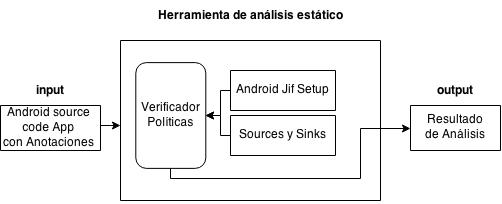
\includegraphics[width=10cm]{desing3-integration.jpg} 
% 	\end{center}
% 	\caption{Herramienta de análisis estático  }
% 	\label{fig:desingInteger}
% \end{figure}

% \begin{figure}[t!]
% 	\begin{center}
% 	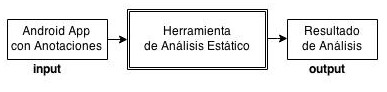
\includegraphics[width=9cm]{desingInOut-3.jpg}
% 	\end{center}
% 	\caption{Herramienta de análisis estático. Ilustra entradas y salidas
% 	esperadas}
% 	\label{fig:desing1}
% \end{figure} 

%color-question para Martín
% \textcolor{blue}{ \textit{P: desde este parrafo hasta el final de la sección,
% está bien dejar esa información así, o sencillamente la podemos omitir?}}\newline
% Luego, la estrategia de evaluación, consiste en verificar si la herramienta
% identifica pérdida de información mediante detección de flujos implícitos. Esto
% debido a que, como se menciona en la descripción del problema, parte importante
% de las propuestas para detección de fuga de información en aplicaciones Android,
% hacen data-flow analysis aplicando técnicas de análisis tainting, y en contraste
% con las técnicas de análisis de flujo de información, las técnicas de análisis
% tainting no necesariamente consideran flujos implícitos. Por tanto, al estar
% basada en JIF, cuyo enfoque de análisis es precisamente flujo de información, se
% esperaría que la herramienta propuesta esté en capacidad de reconocer flujos
% implícitos.
% 
% % Se esperaría que: al realizar análisis de flujo de información aplicando
% % técnicas Security-Typing, la herramienta propuesta, esté en capacidad de
% % reconocer flujos implícitos.\newline
% % Más específicamente, se puede tomar el conjunto de aplicaciones utilizadas como
% % casos de prueba para la detección de flujos implícitos en
% % DroidBench\cite{DroidBenchBenchmarks}, el benchmark de Flowdroid, y analizarlas
% % con la herramienta propuesta.\newline
% 
% Más específicamente, se puede partir de DroidBench\cite{DroidBenchBenchmarks},
% el benchmark de Flowdroid[\ref{FlowDroid-Tool}], tomar el conjunto de
% aplicaciones con que prueban la detección de flujos implícitos, y analizarlas
% con la herramienta propuesta.\newline
% Finalmente estos resultados serían
% comparados con los obtenidos mediante otras herramientas para análisis de fuga
% de información en aplicaciones Android.
% 
% En este orden de ideas, la evaluación de la herramienta propuesta está enfocada
% en: medir recall frente a la detección de flujos implícitos, es decir, medir que
% no genere falsos negativos ante la existencia de fugas de información,
% provenientes de flujos implícitos.\newline
% 
% 


















